%\title{LaTeX Portrait Poster Template}
%%%%%%%%%%%%%%%%%%%%%%%%%%%%%%%%%%%%%%%%%
% a0poster Portrait Poster
% LaTeX Template
% Version 1.0 (22/06/13)
%
% The a0poster class was created by:
% Gerlinde Kettl and Matthias Weiser (tex@kettl.de)
% 
% Adapter by Jens Buysse for Hogeschool Gent
% This template has been downloaded from:
% http://www.LaTeXTemplates.com
%
% License:
% CC BY-NC-SA 3.0 (http://creativecommons.org/licenses/by-nc-sa/3.0/)
%
%%%%%%%%%%%%%%%%%%%%%%%%%%%%%%%%%%%%%%%%%

%----------------------------------------------------------------------------------------
%	PACKAGES AND OTHER DOCUMENT CONFIGURATIONS
%----------------------------------------------------------------------------------------

\documentclass[a0,portrait]{a0poster}

\usepackage{multicol} % This is so we can have multiple columns of text side-by-side
\usepackage{caption}
\usepackage{subcaption}
\columnsep=100pt % This is the amount of white space between the columns in the poster
\columnseprule=3pt % This is the thickness of the black line between the columns in the poster

\usepackage[svgnames]{xcolor} % Specify colors by their 'svgnames', for a full list of all colors available see here: http://www.latextemplates.com/svgnames-colors

\usepackage{times} % Use the times font
%\usepackage{palatino} % Uncomment to use the Palatino font

\usepackage{graphicx} % Required for including images
\graphicspath{{figures/}} % Location of the graphics files
\usepackage{booktabs} % Top and bottom rules for table
\usepackage[font=small,labelfont=bf]{caption} % Required for specifying captions to tables and figures
\usepackage{amsfonts, amsmath, amsthm, amssymb} % For math fonts, symbols and environments
\usepackage{wrapfig} % Allows wrapping text around tables and figures
\usepackage[export]{adjustbox}

\begin{document}

%----------------------------------------------------------------------------------------
%	POSTER HEADER 
%----------------------------------------------------------------------------------------

% The header is divided into two boxes:
% The first is 75% wide and houses the title, subtitle, names, university/organization and contact information
% The second is 25% wide and houses a logo for your university/organization or a photo of you
% The widths of these boxes can be easily edited to accommodate your content as you see fit

\begin{minipage}[t]{0.75\linewidth}
\VeryHuge \color{HoGentAccent1} \textbf{Een slimme spraakassistent bij het verlenen van eerste hulp bij ongevallen} \color{Black}\\ % Title
\Huge\textit{}\\[2.4cm] % Subtitle
\huge \textbf{Reyniers Jorgé, Ronny Pringels, Jens Buysse}\\[0.5cm] % Author(s)
\huge Hogeschool Gent, Valentin Vaerwyckweg 1, 9000 Gent\\[0.4cm] % University/organization
\Large \texttt{jorge.reyniers.w5872@student.hogent.be} \\
\end{minipage}
%
\begin{minipage}[t]{0.25\linewidth}

\includegraphics[width=13cm,right]{figures/HG-woordmerk.png} 

\end{minipage}

\vspace{1cm} % A bit of extra whitespace between the header and poster content

%----------------------------------------------------------------------------------------

\begin{multicols}{2} % This is how many columns your poster will be broken into, a portrait poster is generally split into 2 columns

%----------------------------------------------------------------------------------------
%	ABSTRACT
%----------------------------------------------------------------------------------------

\color{HoGentAccent1} % Navy color for the abstract

\begin{abstract}
Persoonlijke spraakassistenten als Amazon's Alexa, Apple's Siri of de Assistant van Google zijn aan een serieuze opmars bezig in Amerika. Tegenwoordig komen ze ook allemaal met een bijpassende smart speaker waar de spraakassistent is ingebouwd. In België blijft de populariteit nog uit, maar daar kan verandering in komen. Na de aankondiging van Google dat zijn persoonlijke assistent binnenkort een Belgische variant krijgt, sijpelen de eerste toepassingen van de grote bedrijven al binnen. Welk doel, naast winst maken, kan een applicatie voor een spraakassistent nog hebben? Deze bachelorproef was eerst en vooral een zoektocht naar een doel die voor een bepaalde groep een meerwaarde betekent en waar op weinig weerstand wordt gebotst. Een bijzondere doelgroep bleek hiervoor niet de beste optie te zijn. Uiteindelijk is er gekozen om een applicatie te maken die de Vlaming kan helpen bij het verlenen van Eerste Hulp Bij Ongevallen. Veel informatie die nodig is om de applicatie te bouwen is af te leiden uit de recente mobiele applicatie die is gemaakt door het Rode Kruis en die hetzelfde doel heeft.

Er is een literatuuronderzoek geschreven over de wereld van spraaktechnologie. Daaruit blijkt dat spraakassistenten twee noodzakelijke functies hebben, namelijk spraakherkenning en spraaksynthese. Spraakherkenning of Speech-To-Text is gesproken taal omvormen naar voor de computer leesbare taal. Spraaksynthese is net het omgekeerde en is menselijke spraak gevormd door een computer.

Voor de applicatie kan ontwikkeld worden moet er een assistent gekozen worden waarvoor hij wordt gebouwd. Om er niet zomaar één uit te kiezen is er een vergelijkend onderzoek gevoerd naar de kwaliteit van de spraak en spraakherkenning van spraakassistenten.
Uit de resultaten van het eerste deel van het onderzoek worden enkele stellingen bevestigd. Deze tonen aan dat de Nederlandse Google Assistant significant lager scoort op spraakkwaliteit dan de andere twee assistenten. De Engelse assistenten krijgen op elke eigenschap telkens een hogere score dan Google Assistant NL. Tussen de Engelse assistenten onderling is er niet veel verschil te merken. Google Assistent scoort alleen op tempo significant hoger dan Alexa.

Het tweede deel van het onderzoek, het vergelijken van de kwaliteit van de assistenten hun spraakherkenning, was een moeilijkere taak die helaas niet echt in zijn opzet is geslaagd. Ondanks de maatregelen die zijn getroffen om de beïnvloeding van veranderlijke factoren te beperken, is het toch niet gelukt om statistisch correct onderzoek te voeren in het tweede deel. Uit de fouten die bij dit deel zijn gemaakt kunnen er lessen geleerd worden voor onderzoekers die in de toekomst werken met spraakherkenning.

Uiteindelijk is de keuze ondanks de resultaten toch gevallen op de Nederlandstalige Google Assistant. Dit komt omdat de Nederlandse taal een doorslaggevende factor is voor het verlenen van eerste hulp in België. Als er enkel wordt afgegaan op de resultaten van het onderzoek naar de spraakkwaliteit dan is de Google Assistant de favoriet.

Als laatste is er een kort beeld geschetst van hoe een applicatie voor de Google Assistant werkt en hoe die werking kan verlopen bij de specifieke use case van het onderzoek. Het plan is om in de weken na het schrijven van deze bachelorproef een eerste versie te ontwikkelen van de eerstehulp-applicatie voor de Google Assistant. In de toekomst kan deze versie verder getest worden. Feedback van gebruikers kan verwerkt worden en bij interesse van het Rode Kruis kan er mogelijks een samenwerking worden aangegaan.
\end{abstract}
%----------------------------------------------------------------------------------------
%	INTRODUCTION
%----------------------------------------------------------------------------------------

\color{HoGentAccent1} 
\section*{Introductie}
\color{black}
\color{black}
Sinds het bestaan van de computer zijn we het gewoon om externe apparatuur zoals een toetsenbord of muis te hanteren om ermee te communiceren. Dit zorgde doorheen de jaren voor heel wat frustratie en was het voor velen bijna een verplichting om hiermee te leren werken. Toch gebruiken we van mens tot mens een ander soort communicatiemiddel, een manier die ons van nature wordt aangeleerd, de gesproken conversatie.
Een instinctieve kunst die mensen al duizenden jaren onder de knie hebben. Het is één van de eerste en belangrijkste vaardigheden die een kind leert. Een kunst, eigen aan de mens, die nooit hoofdzakelijk is gebruikt als communicatiemiddel met een computer. Toch werd hier al tientallen jaren geleden met geëxperimenteerd. Vandaag de dag komt de verwachting om op dezelfde manier te communiceren met de computer dan als we doen met mensen dichtbij. De laatste jaren is de kwaliteit van spraaksystemen gegroeid door onder meer de doorbraak in neurale netwerken. De spraakkwaliteit heeft zo een niveau bereikt dat de conversatie tussen mens en computer natuurlijk begint aan te voelen.

Het is de reden waarom Apple in 2011 een eerste persoonlijke spraakassistent lanceerde, genaamd Siri. Andere bedrijven volgden snel. Google ontwikkelde de Google Assistant Microsoft bouwde Cortana en Amazon, het bedrijf met één van de grootste webshobs ter wereld, kwam met Alexa op de proppen. De spraakassistenten kunnen tegenwoordig niet alleen gebruikt worden via de smartphone en laptop, maar ook via de Smart Speaker, een slimme luidspreker met ingebouwde spraakassistent.

Beeld het je in. Uw persoonlijke assistent heeft je net gewekt. Wanneer je opstaat, vertelt hij je dat het vandaag 15 graden wordt en overwegend bewolkt. Wanneer je beneden komt overloopt hij de eerste nieuwsfeiten van de dag. Je vindt jouw kamerjas niet en vraagt dan maar aan de assistent om de temperatuur 5 graden te verhogen. Tijdens het ontbijt krijg je nog te horen hoe de huidige verkeerssituatie is naar het werk. Door de lange file ga je pas om 09.07u toekomen op kantoor. Dringend tijd dus om te vertrekken. Assistent, doe jij even de deur voor me op slot?

Je kunt er je wel iets bij voorstellen. Het klinkt allemaal sciencefiction, maar het feit is dat dit al dagelijkse realiteit is. De slimme luidsprekers doen het goed. In de Verenigde Staten hebben één op de vijf volwassenen al toegang tot een smart speaker met stemassistent. De opkomst in België blijft nog even uit, maar lijkt binnenkort te arriveren met de Belgische variant van de Google Assistant. Ook Google Home, de slimme luidspreker van Google zou binnenkort op de Belgische markt verschijnen. In Nederland is het apparaat al langer beschikbaar, namelijk sinds eind oktober 2018.

Omdat de slimme luidspreker nog geen grote vlucht heeft genomen in België zijn het aantal bestaande applicaties voor deze technologie nog schaars. Mijn onderzoek begint met het verhaal over mijn zoektocht naar een gepast doel voor de spraakassistent. Een doel met niet alleen interessante mogelijkheden, maar ook een doel voor een groep die geschikt is om met de huidige middelen onderzocht te worden.

Op 2 april 2019 kondigde het Rode Kruis aan dat het een mobiele applicatie had ontwikkeld om te helpen met het verlenen van eerste hulp bij ongevallen. Ik zag hier direct mijn kans in om naast de mobiele applicatie een toepassing voor de spraakassistent te voorzien.

Het eerste en grootste deel van het onderzoek probeert een antwoord te vinden op volgende onderzoeksvraag: Welke spraakassistent is het meest geschikt om te helpen bij het verlenen van eerste hulp bij ongevallen? Daarna worden de eerste stappen genomen in het ontwikkelen van een EHBO app voor de meest geschikte spraakassistent die kan gebruikt worden door de Vlaming. De Vlaming en niet de Belg, omdat de applicatie om te beginnen in maar één taal zal beschikbaar zijn, het Nederlands.

Spraakherkenning en spraaksynthese zijn twee belangrijke vereisten voor de werking van een spraakassistent. De kwaliteit van deze functies zijn ook belangrijk voor het geven van instructies bij EHBO. Er werd een onderzoek gevoerd naar de kwaliteit van de spraakherkenning en spraaksynthese van drie assistenten. Het gaat om de Nederlandstalige en Engelstalige Google Assistant en de Engelstalige Alexa.
%----------------------------------------------------------------------------------------
%	GEOLOGY
%----------------------------------------------------------------------------------------

\color{Black} % DarkSlateGray color for the rest of the content
\color{HoGentAccent1} 
\section*{Experimenten}
\color{black}

Dit onderzoek probeert verschillen aan te tonen in kwaliteit van spraakherkenning en spraaksynthese tussen de drie assistenten. Dertig participanten stelden drie EHBO-gerelateerde vragen aan elke assistent. Er werd geprobeerd om te meten hoe correct de vragen werden omgevormd van spraak naar tekst. De participanten beoordeelden ook de antwoorden van de assistenten op enkele eigenschappen van spraakkwaliteit.

\begin{center}\vspace{1cm}
    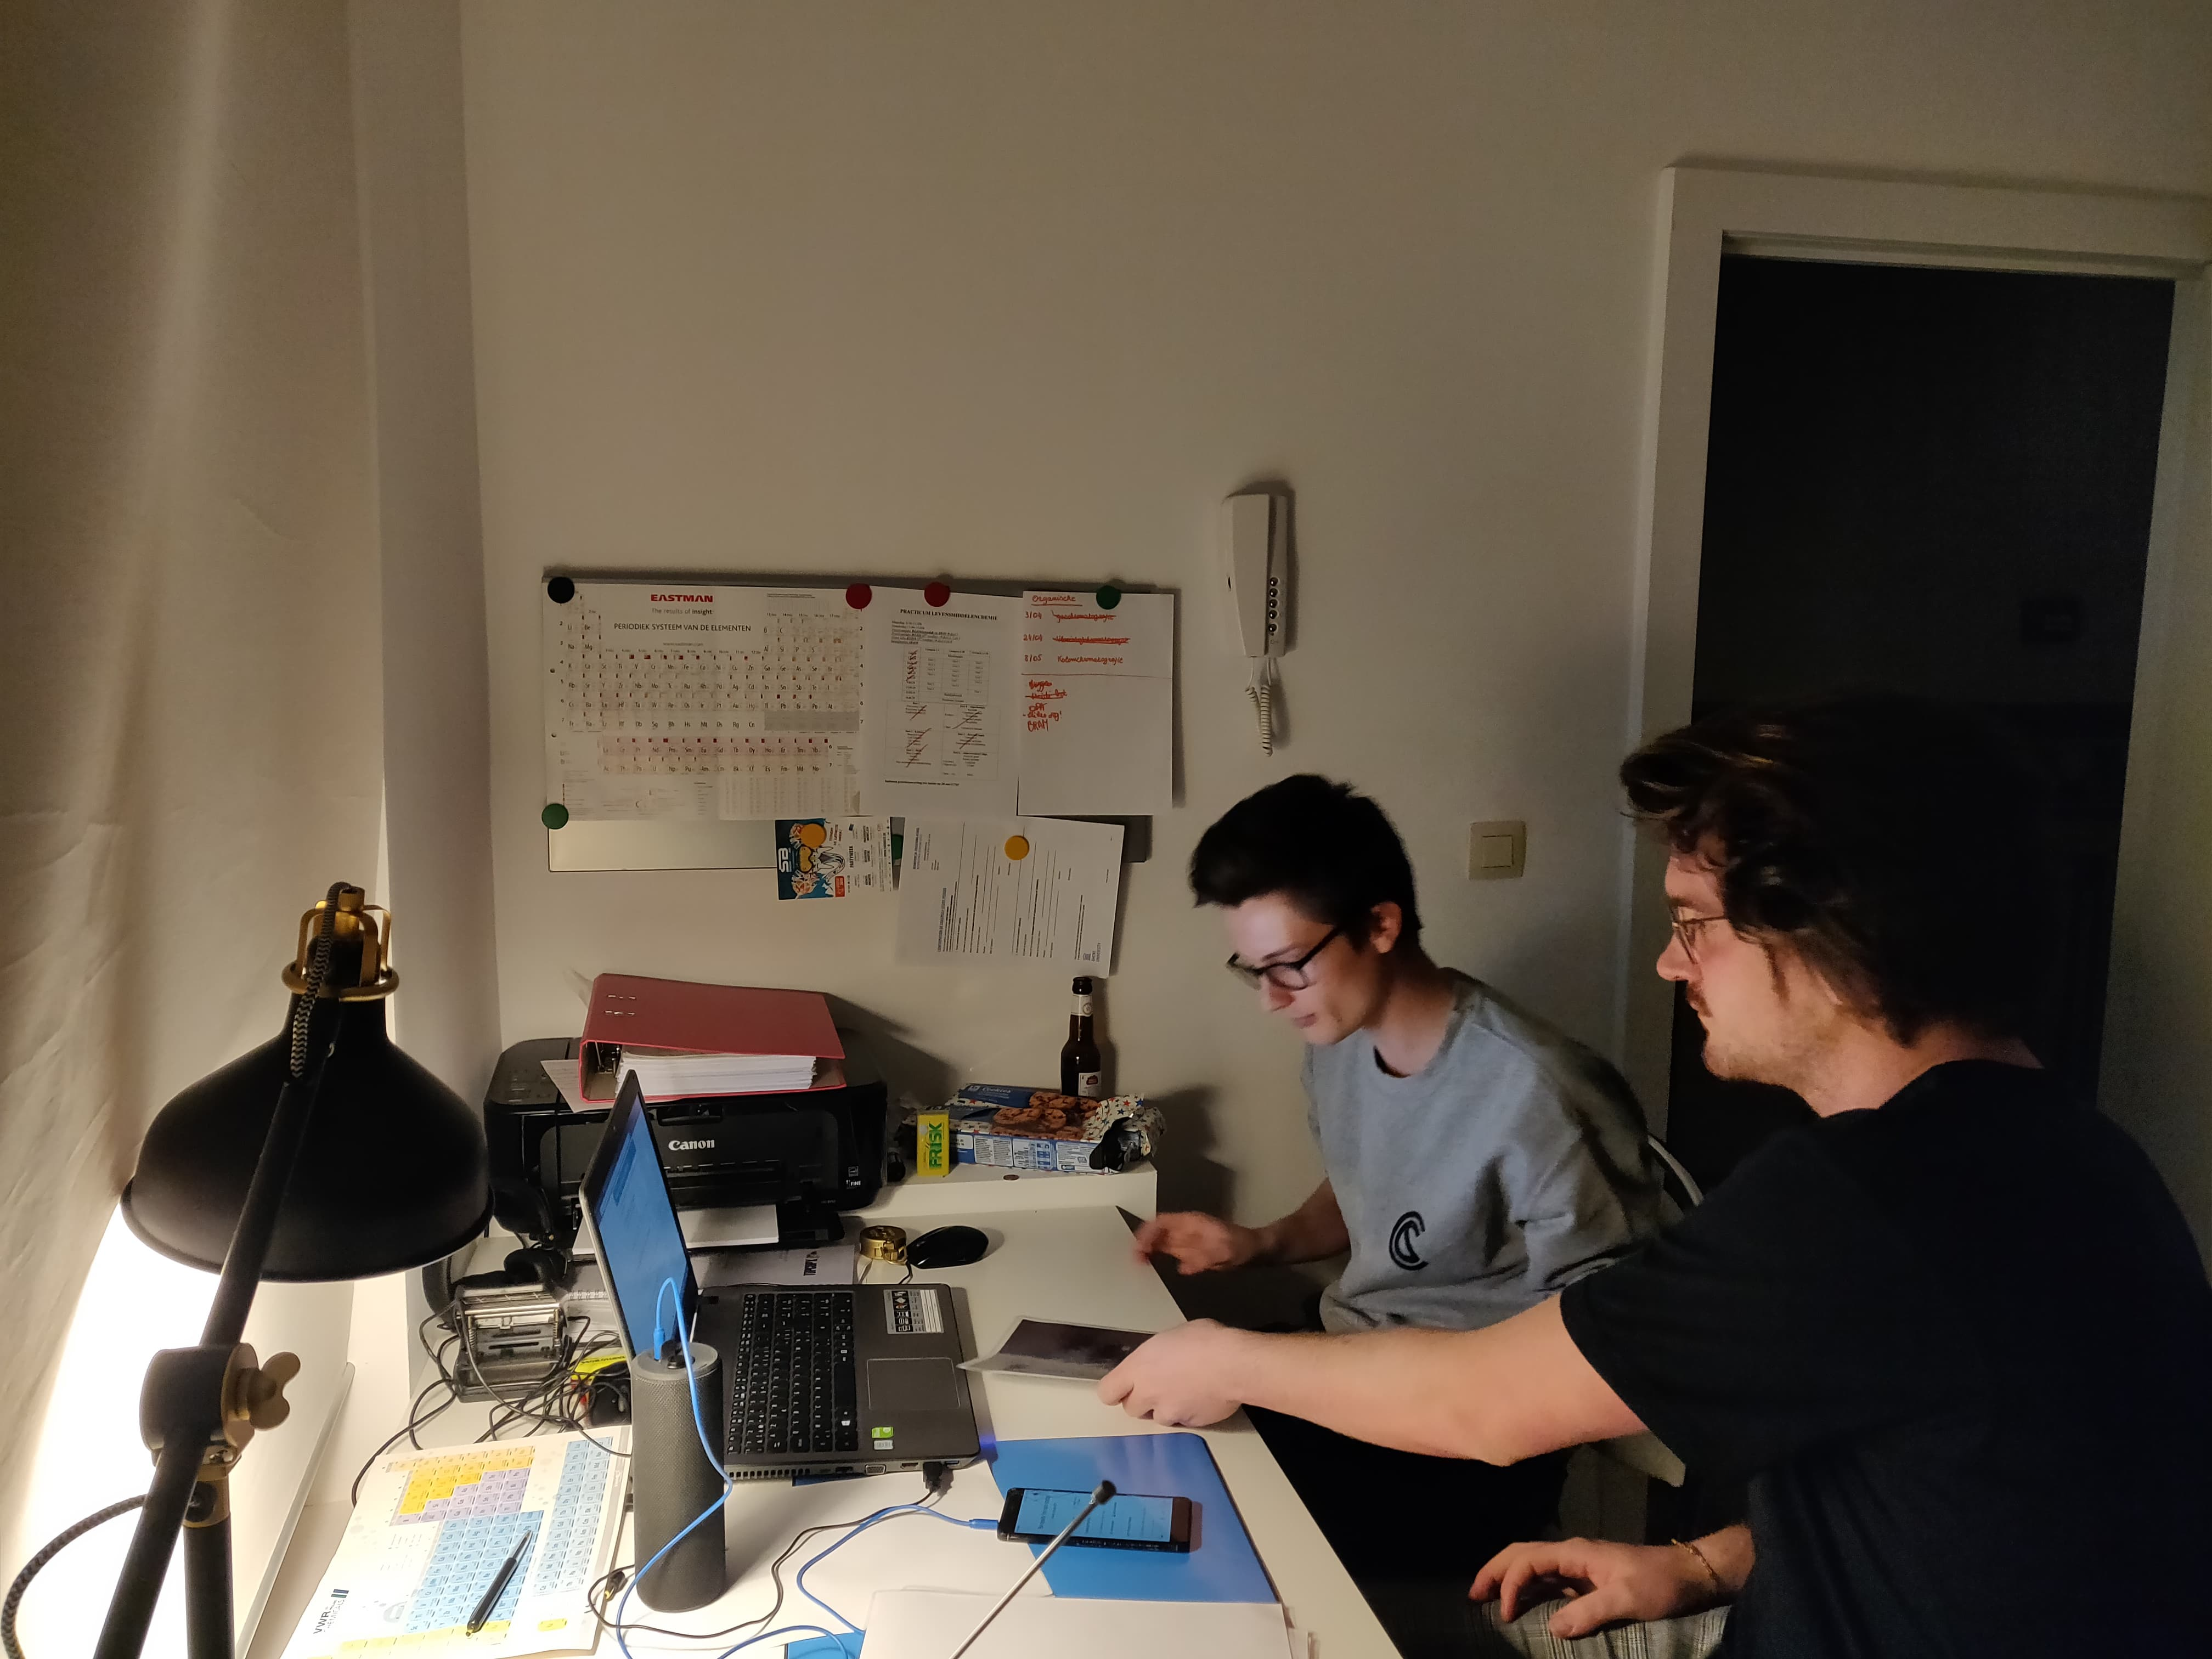
\includegraphics[width=0.44\linewidth]{../bachproef/img/proefafname2}
    \captionof{figure}{\color{HoGentAccent5} Een deelnemer ontvangt de vragen die hij zal stellen aan de assistenten.}
\end{center}\vspace{1cm}

\begin{center}\vspace{1cm}
    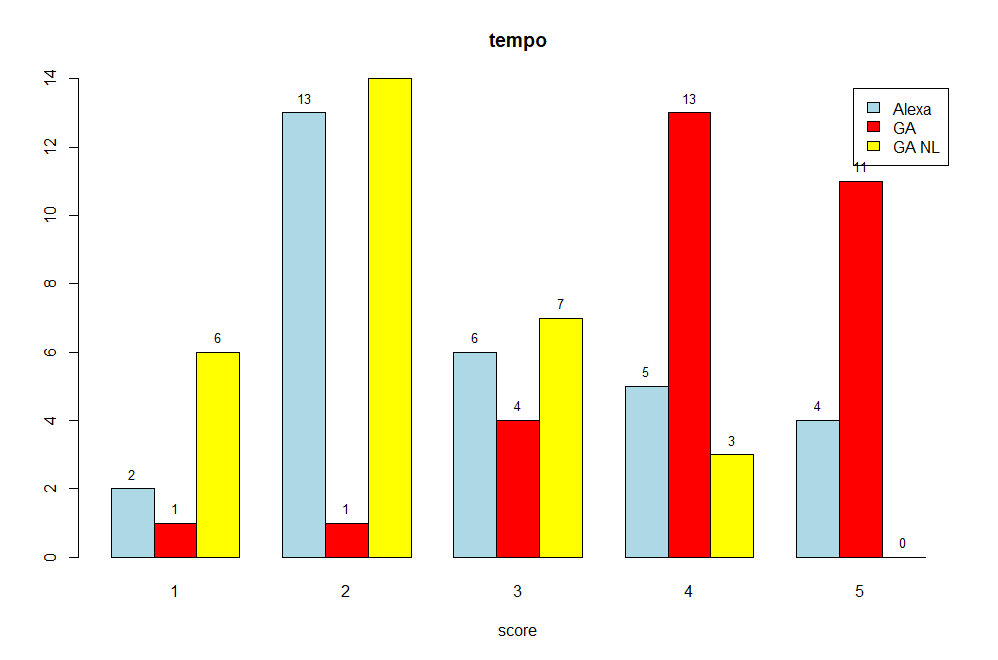
\includegraphics[width=0.44\linewidth]{../onderzoek/onderzoeksresultaten/vergelijking_assistenten_per_eigenschap/barplot/barplot_score_tempo}
    \captionof{figure}{\color{HoGentAccent5} De scores die de deelnemers hebben gegeven op het tempo van de assistenten.}
\end{center}\vspace{1cm}

%------------------------------------------------



\color{HoGentAccent1} 
\section*{Conclusies}
\color{black}
Uit het onderzoek is gebleken dat de algemene spraakkwaliteit van de Engelstalige Alexa en Google Assistant hoger liggen dan die van de Nederlandstalige Google Assistant. Bij elke eigenschap scoorden ze significant hoger dan de Nederlandstalige assistent, met uitzondering van de verstaanbaarheid van Alexa. Voor deze eigenschap kan niet bewezen worden dat de score bij Alexa significant hoger ligt dan bij Google Assistant NL.
Omdat de applicatie moet helpen met eerste hulp verlenen in België is het absoluut nodig dat de assistent Nederlands kan. Google Assistant en Siri zijn de enige twee spraakassistenten die op dit moment een Nederlandse versie hebben. Omdat een ontwikkelaar Siri enkel kan integreren in een bestaande mobiele applicatie gaat de voorkeur eerder naar Google Assistant. Daarnaast is er ook nog het nieuws dat er binnenkort een Vlaamse versie komt van de Google Assistant. Google doet dus uitschijnen dat ze met hun Google Home als eerste willen proberen intrekken in de Vlaamse woonkamers. Deze factoren hebben meegedragen aan het antwoord dat de Google Assistant het meest geschikt is om te helpen bij het verlenen van eerste hulp bij ongevallen. We kunnen besluiten dat er uiteindelijk voor de keuze van de meest geschikte spraakassistent geen rekening is gehouden met de resultaten van het vergelijkend onderzoek.

Dit geldt echter alleen voor België en voor nu. Er kan ook op wereldwijd niveau gekeken worden naar het ontwikkelen van een spraakgestuurde eerstehulp-applicatie. In dit geval kan er wel rekening worden gehouden met de resultaten van het vergelijkend onderzoek voor de landen waar vooral Engels wordt gesproken. De twee Engelstalige assistenten verschillen echter maar aanzienlijk op één eigenschap, namelijk het tempo. De participanten vinden dat Google Assistant op een gepaster tempo praat dan Alexa. Een niet gepast tempo is een tempo dat ervaren wordt als te snel of te traag. Als de meest geschikte spraakassistent alleen o.b.v. deze resultaten wordt gekozen, dan komt Google Assistant opnieuw als winnaar uit de bus komen. De kans bestaat ook dat Alexa of andere spraakassistenten later met een Nederlandse of Vlaamse versie op de markt komen. Het zou interessant zijn om dan dezelfde vergelijking te maken tussen Nederlandstalige assistenten. 

Een correct onderzoek naar de kwaliteit van spraakherkenning verloopt moeilijker dan gedacht. Er is besloten om het aantal fouten die elke assistent heeft gemaakt bij het omvormen van spraak naar tekst niet te tonen of te vergelijken. Waarom dit deel van het onderzoek moeilijk uit te voeren is op een correcte manier, staat beschreven in het onderzoek. Er kunnen lessen uit geleerd worden voor toekomstige onderzoekers die gaan werken in hetzelfde onderzoeksveld.
%----------------------------------------------------------------------------------------
%	FORTHCOMING RESEARCH
%----------------------------------------------------------------------------------------
\color{HoGentAccent1} 
\section*{Toekomstig onderzoek}
\color{black}

Na het schrijven van deze bachelorproef is er het plan om de eerste stappen te zetten in het ontwikkelen van de applicatie. De meest geschikte spraakassistent staat vast en de structuur is getekend. De eerste versie kan ingezet worden om feedback te verzamelen van testgebruikers. Daarnaast kan het Rode Kruis gecontacteerd worden om te polsen wat ze daar van de applicatie vinden. Mogelijks zijn ze geïnteresseerd in een verdere samenwerking voor het ontwikkelen van de applicatie.


%----------------------------------------------------------------------------------------

\end{multicols}
\end{document}